
\section{Results}

The clustering analysis using Latent Dirichlet Allocation (LDA) yielded insights into the patterns
of vulnerabilities as they relate to the Common Vulnerability Scoring System (CVSS) metrics,
particularly the integrity impact metric. While an ideal analysis would involve comparing our
clusters with the assigned Common Weakness Enumeration (CWE), the time constraints and the complex
nature of both our topic-based clusters and the CWE descriptions made automated cross-referencing
unfeasible for the time begin. This limitation presents an opportunity for future research to bridge this gap.

\subsection{Methodology and Presentation}

The primary results of the analysis are presented in graphical form. Each graph shows the
distribution of documents across the three classes of integrity impact (\texttt{NONE}, \texttt{LOW},
\texttt{HIGH}) for the topic cluster that best represents each target class. This approach allows us
to visualize how well this clustering method separates vulnerabilities based on their integrity impact.

\subsection{Integrity Impact Analysis}

The integrity impact metric in CVSS refers to the degree to which a vulnerability, if exploited, could affect the trustworthiness and veracity of data. A high integrity impact implies that data could be significantly corrupted or altered, potentially leading to serious consequences for the affected system or its users.

\subsubsection{\texttt{NONE} Category}
Figure \ref{fig:integrityImpact_20_NONE} shows the distribution for the cluster best representing the \texttt{NONE} category of integrity impact.

\begin{figure}[h]
	\centering
	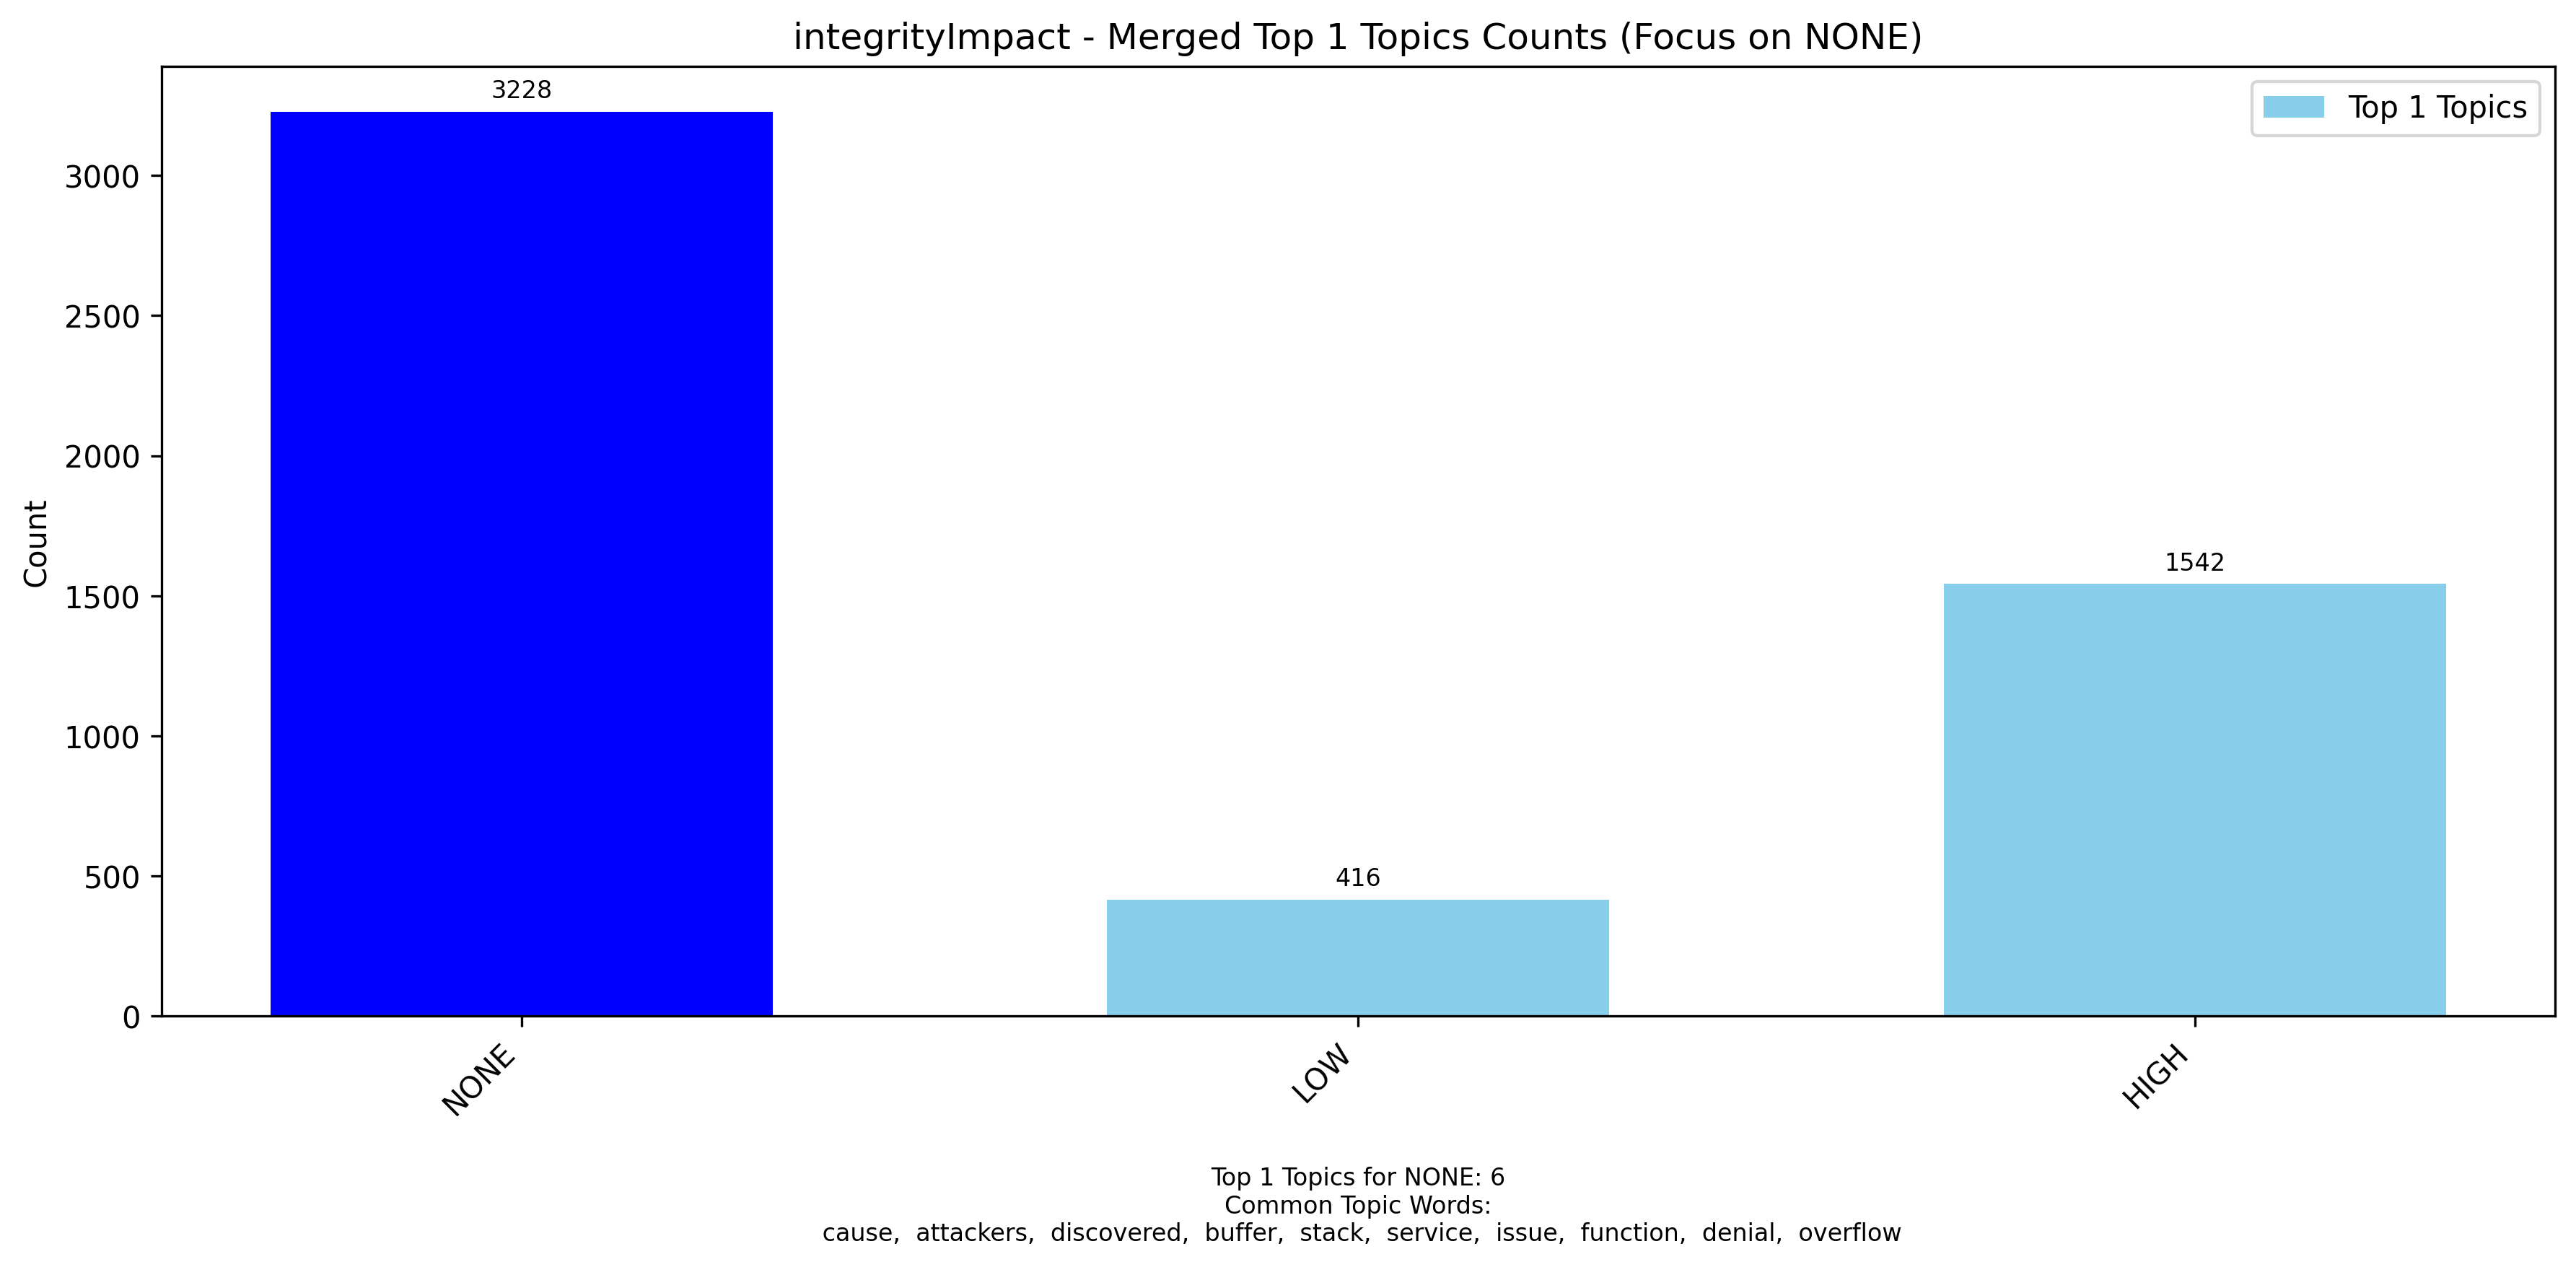
\includegraphics[width=0.8\textwidth]{figures/integrityImpact/merged_top_k_topics_category_focus_counts_integrityImpact_NONE_k1.png}
	\caption{The counts of the documents within the best topic in relation to integrityImpact with target class \texttt{NONE}}
	\label{fig:integrityImpact_20_NONE}
\end{figure}

In this cluster, we observe a predominance of vulnerabilities related to denial of service attacks
and system crashes. While these issues are serious and can affect system availability, they
typically do not directly compromise data integrity. This aligns with the expectations for
vulnerabilities classified as having no integrity impact.

Key findings:
\begin{itemize}
	\item The cluster shows a clear majority of \texttt{NONE}-rated vulnerabilities.
	\item Common terms in this cluster likely include "denial of service", "crash", and "availability".
	\item This result supports the effectiveness of our clustering in identifying vulnerabilities with no integrity impact.
\end{itemize}

\subsubsection{\texttt{LOW} Category}
Figure \ref{fig:integrityImpact_20_LOW} represents the distribution for the cluster best representing the \texttt{LOW} category of integrity impact.

\begin{figure}[h]
	\centering
	\includegraphics[width=0.8\textwidth]{figures/integrityImpact/merged_top_k_topics_category_focus_counts_integrityImpact_LOW_k1.png}
	\caption{The counts of the documents within the best topic in relation to integrityImpact with target class \texttt{LOW}}
	\label{fig:integrityImpact_20_LOW}
\end{figure}

This cluster predominantly features cross-site scripting (XSS) vulnerabilities, often associated with WordPress plugins. These types of vulnerabilities can indeed cause data integrity issues, but they are usually limited in scope, typically affecting individual user interactions rather than compromising the entire application's data integrity.

Key findings:
\begin{itemize}
	\item The cluster shows a majority of \texttt{LOW}-rated vulnerabilities, with some overlap into other categories.
	\item Common terms likely include "cross-site scripting", "XSS", "WordPress", and "plugin".
	\item This cluster aligns with our earlier k-means clustering results, providing validation for our LDA approach.
\end{itemize}

\subsubsection{\texttt{HIGH} Category}
Figure \ref{fig:integrityImpact_20_HIGH} shows the distribution for the cluster best representing the \texttt{HIGH} category of integrity impact.

\begin{figure}[h]
	\centering
	\includegraphics[width=0.8\textwidth]{figures/integrityImpact/merged_top_k_topics_category_focus_counts_integrityImpact_HIGH_k1.png}
	\caption{The counts of the documents within the best topic in relation to integrityImpact with target class \texttt{HIGH}}
	\label{fig:integrityImpact_20_HIGH}
\end{figure}

In this cluster, we see a concentration of SQL injection and database-related vulnerabilities. These
types of attacks have the potential to severely compromise data integrity by allowing unauthorized
modification or corruption of database contents.

Key findings:
\begin{itemize}
	\item The cluster shows a strong representation of \texttt{HIGH}-rated vulnerabilities.

	\item Common terms likely include "SQL injection", "database", and possibly specific database technology names.

	\item The prevalence of these severe vulnerabilities in this cluster aligns with cybersecurity expert expectations for high-impact integrity issues.

\end{itemize}

\subsection{Overall Observations}

\begin{enumerate}

	\item Our clustering approach successfully differentiated between vulnerabilities with varying
	      levels of integrity impact, as evidenced by the distinct profiles of each cluster.

	\item The results align well with expert knowledge in the field of cybersecurity, suggesting
	      that our unsupervised learning approach can capture meaningful patterns in vulnerability
	      data.

	\item While our current analysis provides a static view of the vulnerability landscape, the
	      temporal aspect of the data presents an opportunity for future research. Analyzing how these
	      clusters and trends have evolved over time could provide additional insights into the
	      changing nature of cybersecurity threats.

	\item The overlap between categories in some clusters (particularly visible in the \texttt{LOW}
	      category) highlights the complexity of vulnerability classification and the potential for
	      ambiguity in CVSS scoring.

\end{enumerate}

These results demonstrate the potential of unsupervised learning techniques, particularly LDA, in
analyzing and categorizing vulnerability data. By revealing natural groupings and associations
between types of vulnerabilities and their impacts, this approach can inform more nuanced strategies
for vulnerability management and potentially improve automated CVSS scoring systems.

\subsection{Confidentiality Impact Analysis}

The integrity impact metric in CVSS refers to the degree to which a vulnerability, if exploited,
could affect the trustworthiness and veracity of data. A high integrity impact implies that data
could be significantly corrupted or altered, potentially leading to serious consequences for the
affected system or its users.

\subsubsection{\texttt{NONE} Category}

Figure \ref{fig:confidentialityImpact_20_NONE} shows the distribution for the cluster best
representing the \texttt{NONE} category of integrity impact.

\begin{figure}[h]
	\centering
	\includegraphics[width=0.8\textwidth]{figures/confidentialityImpact/}
	\caption{The counts of the documents within the best topic in relation to confidentialityImpact with target class \texttt{NONE}}
	\label{fig:confidentialityImpact_20_NONE}
\end{figure}

In this cluster, we observe a predominance of vulnerabilities related to denial of service attacks
and system crashes. While these issues are serious and can affect system availability, they
typically do not directly compromise data integrity. This aligns with the expectations for
vulnerabilities classified as having no integrity impact.

Key findings:
\begin{itemize}
	\item The cluster shows a clear majority of \texttt{NONE}-rated vulnerabilities.
	\item Common terms in this cluster likely include "denial of service", "crash", and "availability".
	\item This result supports the effectiveness of our clustering in identifying vulnerabilities with no integrity impact.
\end{itemize}

\subsubsection{\texttt{LOW} Category}
Figure \ref{fig:confidentialityImpact_20_LOW} represents the distribution for the cluster best representing the \texttt{LOW} category of integrity impact.

\begin{figure}[h]
	\centering
	\includegraphics[width=0.8\textwidth]{figures/confidentialityImpact/merged_top_k_topics_category_focus_counts_integrityImpact_LOW_k1.png}
	\caption{The counts of the documents within the best topic in relation to confidentialityImpact with target class \texttt{LOW}}
	\label{fig:confidentialityImpact_20_LOW}
\end{figure}

This cluster predominantly features cross-site scripting (XSS) vulnerabilities, often associated with WordPress plugins. These types of vulnerabilities can indeed cause data integrity issues, but they are usually limited in scope, typically affecting individual user interactions rather than compromising the entire application's data integrity.

Key findings:
\begin{itemize}
	\item The cluster shows a majority of \texttt{LOW}-rated vulnerabilities, with some overlap into other categories.
	\item Common terms likely include "cross-site scripting", "XSS", "WordPress", and "plugin".
	\item This cluster aligns with our earlier k-means clustering results, providing validation for our LDA approach.
\end{itemize}

\subsubsection{\texttt{HIGH} Category}
Figure \ref{fig:confidentialityImpact_20_HIGH} shows the distribution for the cluster best representing the \texttt{HIGH} category of integrity impact.

\begin{figure}[h]
	\centering
	\includegraphics[width=0.8\textwidth]{figures/confidentialityImpact/merged_top_k_topics_category_focus_counts_integrityImpact_HIGH_k1.png}
	\caption{The counts of the documents within the best topic in relation to confidentialityImpact with target class \texttt{HIGH}}
	\label{fig:confidentialityImpact_20_HIGH}
\end{figure}

In this cluster, we see a concentration of SQL injection and database-related vulnerabilities. These types of attacks have the potential to severely compromise data integrity by allowing unauthorized modification or corruption of database contents.

Key findings:
\begin{itemize}
	\item The cluster shows a strong representation of \texttt{HIGH}-rated vulnerabilities.
	\item Common terms likely include "SQL injection", "database", and possibly specific database technology names.
	\item The prevalence of these severe vulnerabilities in this cluster aligns with cybersecurity expert expectations for high-impact integrity issues.
\end{itemize}

\subsection{Overall Observations}

\begin{enumerate}
	\item Our clustering approach successfully differentiated between vulnerabilities with varying levels of integrity impact, as evidenced by the distinct profiles of each cluster.

	\item The results align well with expert knowledge in the field of cybersecurity, suggesting that our unsupervised learning approach can capture meaningful patterns in vulnerability data.

	\item While our current analysis provides a static view of the vulnerability landscape, the temporal aspect of the data presents an opportunity for future research. Analyzing how these clusters and trends have evolved over time could provide additional insights into the changing nature of cybersecurity threats.

	\item The overlap between categories in some clusters (particularly visible in the \texttt{LOW} category) highlights the complexity of vulnerability classification and the potential for ambiguity in CVSS scoring.
\end{enumerate}

These results demonstrate the potential of unsupervised learning techniques, particularly LDA, in analyzing and categorizing vulnerability data. By revealing natural groupings and associations between types of vulnerabilities and their impacts, this approach can inform more nuanced strategies for vulnerability management and potentially improve automated CVSS scoring systems.
\subsection{Cluster Merging and Refinement}

In an attempt to enhance class representation and potentially improve the overall performance of our topic model, we explored the concept of merging related clusters. This process involved several steps:

\begin{itemize}
	\item Identifying clusters with semantic similarity or overlapping representation of CVSS classes.
	\item Merging these clusters by combining their topic-word distributions and reassigning documents.
	\item Recalculating class representation metrics for the merged clusters.
	\item Comparing the performance of the merged model to the original in terms of:
	      \begin{itemize}
		      \item Overall topic coherence
		      \item Clarity of class representation
		      \item Interpretability of resulting topics
	      \end{itemize}
\end{itemize}

\subsubsection{Methodology}

Our approach to cluster merging was based on a simple similarity metric between topic-word distributions. Clusters were merged if their similarity exceeded a predefined threshold. While this method is straightforward to implement, it is admittedly crude and may not capture all the nuances of semantic similarity between topics.

It's worth noting that more sophisticated approaches exist. For instance, Neuhaus \& Zimmerman (2010)~\cite{cve_topic_modelling} merged clusters based on the similarity of the topic words found by their model. This approach, which we intend to explore in future work, potentially offers a more nuanced way of identifying truly related topics.

\subsubsection{Results}

To illustrate the effects of cluster merging, we present the following figures:

% Insert figures here
% \begin{figure}[h]
% \centering
% \includegraphics[width=0.8\textwidth]{path_to_original_cluster_figure}
% \caption{Distribution of CVSS classes in original clusters}
% \label{fig:original_clusters}
% \end{figure}

% \begin{figure}[h]
% \centering
% \includegraphics[width=0.8\textwidth]{path_to_merged_cluster_figure}
% \caption{Distribution of CVSS classes in merged clusters}
% \label{fig:merged_clusters}
% \end{figure}

Contrary to our initial expectations, the process of merging clusters did not lead to improved
results. Instead, I observed the following effects:

\begin{itemize}
	\item \textbf{Decreased Cluster Purity:} The merged clusters showed a higher mix of different CVSS classes compared to the original clusters. This indicates that the merging process combined not only semantically similar vulnerabilities but also those with different CVSS ratings.

	\item \textbf{Reduced Interpretability:} The larger, merged clusters became more difficult to interpret. The defining characteristics of individual clusters became diluted, making it harder to assign clear semantic meanings to each cluster.

	\item \textbf{Loss of Granularity:} While the original clusters often represented specific types of vulnerabilities or attack vectors, the merged clusters tended to group broader categories together, losing some of the nuanced distinctions that were valuable in the original model.

	\item \textbf{Decreased Topic Coherence:} The overall topic coherence of the model decreased after merging, suggesting that the combined topics were less internally consistent than the original, more granular topics.
\end{itemize}

\subsubsection{Interpretation and Future Directions}

These results suggest that our initial clustering approach was already capturing meaningful
distinctions between different types of vulnerabilities and their associated CVSS ratings. The
process of merging clusters, at least with the current methodology, appears to obscure these
distinctions rather than enhance them.

However, this does not necessarily mean that cluster merging is inherently unhelpful. Instead, it suggests that more sophisticated merging strategies may be needed to preserve the valuable information captured in the original clusters while still allowing for the combination of truly related topics.

For future work, I propose the following directions:

\begin{itemize}
	\item Implementing the cluster merging approach of Neuhaus \& Zimmerman (2010), which focuses on the similarity of topic words rather than overall distribution similarity.
	\item Exploring hierarchical topic modeling approaches, which might allow for the representation of both fine-grained and broader topic categories simultaneously.
	\item Investigating dynamic topic modeling techniques to capture how vulnerability types and their CVSS ratings evolve over time, potentially revealing patterns in how initially distinct vulnerability categories merge or diverge over time.
\end{itemize}

